% !TEX program = xelatex
% ============================================================
%  财富庄园 · Wealth Manor —— 企划书（三、产品与服务）
%  工行APP游戏化智能理财与个人财产管理平台
%  编译：latexmk -xelatex main.tex
% ============================================================
\documentclass[12pt,a4paper]{ctexart}

% ---------- 宏包 ----------
\usepackage[margin=2.4cm,top=2.8cm,bottom=2.8cm]{geometry}
\usepackage{amsmath}
\usepackage{graphicx}
\usepackage{booktabs}
\usepackage[table]{xcolor}
\usepackage{array}
\usepackage{longtable}
\usepackage{tikz}
\usetikzlibrary{positioning,arrows.meta,shadows,calc}
\usepackage{enumitem}
\usepackage{fancyhdr}
\usepackage{hyperref}
\usepackage{float}

% ---------- 颜色 ----------
\definecolor{icbcred}{HTML}{C8102E}
\definecolor{manorgreen}{HTML}{4E8C4E}
\definecolor{rowgray}{HTML}{F5F5F5}

% ---------- 页眉页脚 ----------
\pagestyle{fancy}
\fancyhf{}
\fancyhead[C]{\small\color{icbcred}财富庄园·Wealth Manor —— 企划书（三、产品与服务）}
\fancyfoot[C]{\small\thepage}
\renewcommand{\headrulewidth}{0.4pt}

% ---------- 超链接样式 ----------
\hypersetup{
  colorlinks=true,
  linkcolor=icbcred,
  urlcolor=manorgreen,
  pdftitle={财富庄园企划书——产品与服务},
  pdfauthor={财富庄园团队}
}

% ---------- 表格行着色 ----------
\rowcolors{2}{rowgray}{white}

% ---------- 列表间距 ----------
\setlist{itemsep=2pt,topsep=3pt}
\linespread{1.25}

\begin{document}

% ============================================================
% 三、产品与服务
% ============================================================
\section{产品与服务}

% ---------------- 3.1 平台理念 ----------------
\subsection{平台理念}

\subsubsection{使命与愿景}
财富庄园的使命是\textbf{"让理财像玩游戏一样简单，让每个人都能看清自己的全部财富版图"}。
平台相信：理财不应是少数人的专业游戏，而应是每个人日常生活的组成部分。
通过把抽象的金融概念翻译成用户熟悉的"种植—生长—收获"语言，把分散的资产
汇聚成一棵看得见的"财富树"，理财从一件"该做但不想做"的事，变成一件
"想主动去做"的事。

\subsubsection{三大设计原则}
\begin{enumerate}
  \item \textbf{行为即游戏，游戏即成长}：每一种真实理财行为（购买、定投、查看、
        学习）都对应庄园中的确定性反馈（种子、生长加速、金币、经验），
        让好习惯即时获得正反馈；
  \item \textbf{数据真实，绝不模拟}：庄园的一切状态都映射自用户的真实资产——
        植物生长对应持仓收益，天气对应市场行情，荣誉点只来自真实理财行为，
        游戏是"真实财富的可视化界面"而非虚拟世界；
  \item \textbf{普惠与合规并重}：面向零基础用户降低门槛，同时严守金融合规红线——
        游戏积分不可兑换现金、理财产品购买走正规流程、资产数据仅展示不存储明细。
\end{enumerate}

\subsubsection{目标用户与产品定位}
\begin{table}[htbp]
\centering
\begin{tabular}{p{3cm}p{9.5cm}}
\toprule
\textbf{维度} & \textbf{说明} \\
\midrule
核心用户 & 18--35岁年轻客群：理财新手、基金定投用户、有房有贷的工薪族 \\
产品定位 & 工行APP内的"理财入口 + 财富仪表盘 + 陪伴式游戏"三位一体模块 \\
差异化 & 与蚂蚁森林（纯公益）、记账类产品（纯记录）、传统理财专区（纯工具）形成本质区隔 \\
\bottomrule
\end{tabular}
\caption{目标用户与产品定位}
\end{table}

% ---------------- 3.2 技术架构 ----------------
\subsection{技术架构}

\subsubsection{总体分层架构}
平台采用"客户端—网关—BFF聚合—微服务—数据层"五层架构，部署于工行金融云，
与工行现有账户体系、产品中心通过API网关对接：

\begin{figure}[htbp]
\centering
\footnotesize
\begin{tikzpicture}[
  layer/.style={draw=icbcred!60, fill=icbcred!6, rounded corners=3pt,
    minimum width=14.8cm, align=center, text width=14.4cm,
    inner sep=6pt},
  box/.style={draw=black!55, fill=white, rounded corners=2pt,
    minimum height=8mm, minimum width=3.2cm, align=center, font=\scriptsize},
  arr/.style={-{Stealth[length=2.5mm]}, thick, draw=black!70}
]
% 客户端层
\node[layer] (client) at (0,0) {
  客户端 —— 工行APP（iOS / Android）\\
  \begin{tikzpicture}
    \node[box] (g1) {游戏引擎\\Cocos Creator 3.x};
    \node[box, right=8mm of g1] (g2) {资产看板\\原生 H5};
    \node[box, right=8mm of g2] (g3) {AI 助手对话\\NLP 服务};
    \node[box, right=8mm of g3] (g4) {入口与推送\\Banner / Push};
  \end{tikzpicture}
};
% 网关层
\node[layer, below=5mm of client] (gw) {
  统一 API 网关 —— 鉴权（工行统一认证 + 生物识别）/ 限流 / 熔断 / 国密 TLS
};
% BFF层
\node[layer, below=5mm of gw] (bff) {
  BFF 聚合层（Backend For Frontend）\\
  \begin{tikzpicture}
    \node[box] (b1) {游戏 BFF\\庄园状态聚合};
    \node[box, right=8mm of b1] (b2) {资产聚合 BFF\\多源资产视图};
    \node[box, right=8mm of b2] (b3) {AI 推荐 BFF\\建议/问答编排};
    \node[box, right=8mm of b3] (b4) {社交 BFF\\好友/排行};
  \end{tikzpicture}
};
% 微服务层
\node[layer, below=5mm of bff] (micro) {
  微服务层\\
  \begin{tikzpicture}
    \node[box] (m1) {游戏服务\\庄园/种子/任务/商城};
    \node[box, right=6mm of m1] (m2) {资产服务\\全资产/估值/趋势};
    \node[box, right=6mm of m2] (m3) {AI 引擎\\风评/配置建议/知识};
    \node[box, right=6mm of m3] (m4) {用户服务\\认证/好友/积分};
    \node[box, below=3mm of m1] (m5) {OCR 服务\\证件/合同识别};
    \node[box, below=3mm of m2] (m6) {市场数据\\行情/估值API};
    \node[box, below=3mm of m3] (m7) {消息服务\\推送/活动通知};
    \node[box, below=3mm of m4] (m8) {数据统计\\行为分析/AB测试};
  \end{tikzpicture}
};
% 数据层
\node[layer, below=5mm of micro] (data) {
  数据层\\
  \begin{tikzpicture}
    \node[box] (d1) {MySQL\\主数据};
    \node[box, right=8mm of d1] (d2) {Redis\\缓存/排行榜};
    \node[box, right=8mm of d2] (d3) {ElasticSearch\\搜索/日志};
    \node[box, right=8mm of d3] (d4) {Kafka\\消息队列};
  \end{tikzpicture}
  \\[1mm]
  \begin{tikzpicture}
    \node[box, minimum width=14.4cm] (d5) {数据仓库 Hive / ClickHouse —— 用户画像 · 行为分析 · 收益归因};
  \end{tikzpicture}
};
% 层间箭头
\draw[arr] (client.south) -- (gw.north);
\draw[arr] (gw.south) -- (bff.north);
\draw[arr] (bff.south) -- (micro.north);
\draw[arr] (micro.south) -- (data.north);
\end{tikzpicture}
\caption{财富庄园总体分层架构}
\end{figure}

\subsubsection{核心技术选型}
\begin{table}[htbp]
\centering
\begin{tabular}{p{3cm}p{4.5cm}p{5cm}}
\toprule
\textbf{领域} & \textbf{生产环境选型} & \textbf{选型理由} \\
\midrule
游戏引擎 & Cocos Creator 3.x & 包体增量仅约8MB，支持H5与原生混合渲染，适合2D休闲玩法，可经WebView + JSBridge集成至工行APP \\
资产看板 & Vue 3 + 原生H5 & 图表交互丰富、跨端复用、与游戏模块同构技术栈 \\
后端服务 & Spring Cloud 微服务（工行金融云） & 银行级高可用、与行内现有服务治理体系一致 \\
AI能力 & 大模型 + 规则引擎双引擎 & 大模型负责对话与生成式建议，规则引擎兜底合规与可解释性 \\
数据存储 & MySQL + Redis + ES + Kafka & 主数据/缓存排行榜/检索日志/异步解耦各司其职 \\
安全 & 国密SM2/SM4 + TLS 1.3 & 满足金融行业国密改造要求 \\
\bottomrule
\end{tabular}
\caption{核心技术选型}
\end{table}

\subsubsection{核心数据模型}
数据模型划分为\textbf{用户资产域}与\textbf{游戏域}两大领域：

\begin{table}[htbp]
\centering
\begin{tabular}{p{3.2cm}p{4.2cm}p{5.2cm}}
\toprule
\textbf{实体} & \textbf{关键字段} & \textbf{说明} \\
\midrule
User（用户） & id, phone, icbc\_uid, risk\_level & 与工行统一用户体系关联，风评等级驱动产品推荐 \\
AssetAccount（资产账户） & source, account\_type, balance, sync\_type, last\_sync & 多来源资产账户：工行/他行/证券/不动产/其他；支持自动/扫码/OCR/手动四种同步方式 \\
AssetSnapshot（资产快照） & date, total\_net\_worth, breakdown\_json & 每日打点，支撑趋势图与收益归因 \\
FinancialGoal（理财目标） & goal\_type, target\_amount, target\_date, linked\_products & 购房/教育/养老等场景化目标 \\
Manor（庄园） & name, style, level, exp, coins, diamonds & 庄园主档：等级经验、双币种积分 \\
Plot（地块） & plot\_type, position, unlocked & 花园/果园/温室/仓库四类地块 \\
Plant（植物） & species, linked\_product\_id, growth\_stage, mature\_date, yield\_rate & 每株植物关联一笔真实理财产品，收益率映射果实品质 \\
TaskInstance（任务实例） & task\_type, progress, target, reward\_claimed & 任务进度与领取状态 \\
SocialRelation（社交关系） & user\_a, user\_b, interact\_type & 好友关系与浇水/互访/PK记录 \\
\bottomrule
\end{tabular}
\caption{核心数据模型（ER概要）}
\end{table}

\subsubsection{API设计一览}
所有接口以 \texttt{/api/v1} 为前缀，遵循RESTful规范，统一返回
\texttt{\{code, message, data\}} 结构：

\begin{table}[htbp]
\centering
\begin{tabular}{p{4.5cm}p{8cm}}
\toprule
\textbf{接口分组} & \textbf{代表接口} \\
\midrule
资产管理 & \texttt{POST /assets/import}、\texttt{GET /assets/overview}、
\texttt{GET /assets/snapshot/trend}、\texttt{GET /assets/health-score}、
\texttt{POST /assets/optimize} \\
游戏系统 & \texttt{POST /manor/create}、\texttt{GET /manor/state}、
\texttt{POST /manor/plant/seed}、\texttt{POST /manor/plant/\{id\}/harvest}、
\texttt{GET /manor/weather}、\texttt{GET /manor/leaderboard} \\
任务与商城 & \texttt{GET /manor/tasks}、\texttt{POST /manor/tasks/\{id\}/claim}、
\texttt{GET /manor/shop/items}、\texttt{POST /manor/shop/buy} \\
社交系统 & \texttt{POST /manor/social/visit}、\texttt{POST /manor/social/water} \\
AI服务 & \texttt{POST /ai/risk-assessment}、\texttt{GET /ai/portfolio-advice}、
\texttt{POST /ai/goal-planning}、\texttt{POST /ai/chat} \\
知识答题 & \texttt{GET /quiz/questions}、\texttt{POST /quiz/submit} \\
\bottomrule
\end{tabular}
\caption{API设计一览（v1）}
\end{table}

\subsubsection{安全设计}
\begin{table}[htbp]
\centering
\begin{tabular}{p{3cm}p{9.5cm}}
\toprule
\textbf{层面} & \textbf{措施} \\
\midrule
身份认证 & 工行APP统一认证 + 生物识别（指纹/人脸） \\
数据传输 & TLS 1.3 + 国密SM2/SM4 全链路加密 \\
资产数据 & 仅展示不存储明细，外部资产授权后实时获取、不落库 \\
OCR处理 & 本地OCR优先（房产证等隐私件），云端OCR加密传输 \\
防沉迷 & 每日游戏时长限制30分钟，真实理财行为不受限 \\
合规红线 & 游戏积分不可兑换现金；理财产品购买走正规金融流程；收益展示不作收益承诺 \\
\bottomrule
\end{tabular}
\caption{安全与合规设计}
\end{table}

% ---------------- 3.3 功能介绍 ----------------
\subsection{功能介绍}

平台由\textbf{游戏化理财体验}与\textbf{智能全资产看板}两大核心模块构成，
二者通过"真实资产数据驱动游戏状态"这一桥梁深度融合。

\subsubsection{模块一：游戏化理财体验}

\textbf{（1）种植系统——理财产品购买映射}

用户购买理财产品即在庄园获得对应"种子"，产品类型决定种子品类与生长周期：

\begin{table}[htbp]
\centering
\begin{tabular}{p{2.6cm}p{3.6cm}p{3.2cm}p{3.2cm}}
\toprule
\textbf{种子品类} & \textbf{对应产品} & \textbf{生长周期} & \textbf{游戏反馈} \\
\midrule
花朵种子 & 稳健型（存款/货币基金） & 7天开花 & 低波动，稳定产出 \\
果树种子 & 进取型（股票/基金/ETF） & 30天结果 & 果实随收益涨跌 \\
林木种子 & 长期型（养老/教育金） & 180天成材 & 时间复利，成材丰产 \\
杂交种子 & 策略型（组合/投顾） & 自定义周期 & 个性化配置 \\
\bottomrule
\end{tabular}
\caption{种植系统：理财产品与种子的映射}
\end{table}

\begin{itemize}
  \item 收益率 = 果实品质/数量；提前赎回 = 植物枯萎（视觉惩罚+少量扣分）；
        到期赎回 = 丰收（奖励积分 + 庄园经验）。
\end{itemize}

\textbf{（2）任务系统——理财行为引导}

\begin{table}[htbp]
\centering
\begin{tabular}{p{2.6cm}p{6cm}p{4cm}}
\toprule
\textbf{任务类型} & \textbf{示例} & \textbf{奖励} \\
\midrule
日常任务 & 每日查看资产看板 & 浇水券 $\times$1 \\
周任务 & 完成一次风险评估 & 化肥 $\times$1 \\
月任务 & 资产配置多样性$\geq$3类 & 稀有种子 $\times$1 \\
成就任务 & 连续定投3个月 & 庄园扩建许可 \\
知识任务 & 理财知识答题（5题/天） & 金币 + 徽章碎片 \\
\bottomrule
\end{tabular}
\caption{庄园任务系统}
\end{table}

\textbf{（3）天气系统——市场行情映射}

\begin{table}[htbp]
\centering
\begin{tabular}{p{2.6cm}p{4.5cm}p{5.5cm}}
\toprule
\textbf{天气} & \textbf{触发条件} & \textbf{游戏表现} \\
\midrule
晴天 & 当日持仓盈利 & 阳光明媚，植物加速生长 \\
雨天 & 当日持仓亏损 & 庄园下雨，植物略萎靡（不死亡） \\
多云 & 持仓持平 & 正常生长 \\
彩虹 & 单日收益创新高 & 彩虹特效 + 限时稀有商店 \\
暴风雨 & 市场大跌（$>$3\%） & 弹出"加仓机会"提示与陪伴安抚 \\
\bottomrule
\end{tabular}
\caption{天气系统：行情与情绪的双向映射}
\end{table}

\textbf{（4）社交系统}：好友庄园互访浇水（双方各获金币）、月度资产配置合理性
评分PK、好友间理财知识联赛。

\textbf{（5）庄园装扮商店}：金币/钻石/荣誉点三轨积分兑换建筑皮肤、植物品种、
背景音乐、庄园装饰与称号徽章；其中\textbf{荣誉点仅来自真实理财行为}，
确保游戏价值与真实财富行为强绑定。

\textbf{（6）财富树——资产配置可视化}：庄园中心的财富树是用户全部资产的
"生物化仪表盘"——树干粗细=总资产，不同分支=不同资产类别（存存宽叶=现金存款、
红色果实=股票权益、金色花朵=基金、坚固树根=不动产），树冠大小=净资产总额，
树叶茂密度=资产配置均衡度，树的高度=长期财富增长趋势。

\subsubsection{模块二：智能全资产看板}

\textbf{（1）全资产导入体系}——四种通道覆盖全部资产形态：

\begin{table}[htbp]
\centering
\begin{tabular}{p{2.8cm}p{3.4cm}p{6.4cm}}
\toprule
\textbf{导入方式} & \textbf{适用资产} & \textbf{技术实现} \\
\midrule
自动同步 & 工行内存款/理财/基金/贷款/信用卡 & 行内账户体系直连，免操作 \\
扫码/授权导入 & 他行余额、证券持仓、互联网平台资产 & 银联授权 + 券商截图OCR + 平台开放授权 \\
拍照OCR识别 & 房产证、车辆登记证、保单 & OCR提取 + 房天下/链家、二手车估值API自动估价 \\
手动/智能录入 & 海外资产、数字资产、贵重物品 & 手动录入 + 汇率自动换算 \\
\bottomrule
\end{tabular}
\caption{全资产四通道导入体系}
\end{table}

\textbf{（2）智能看板}：总净资产、今日变动、资产配置饼图、近30天净资产趋势、
月度收支现金流一屏呈现；点击任意资产类别可下钻至账户明细。

\textbf{（3）AI智能分析}：

\begin{table}[htbp]
\centering
\begin{tabular}{p{3.4cm}p{9.2cm}}
\toprule
\textbf{功能} & \textbf{说明} \\
\midrule
资产健康度评分 & 0--100分，综合评估流动性、安全性、收益性三维度 \\
配置建议 & 基于年龄/风险偏好/市场环境给出调仓建议，支持"一键优化" \\
收益归因 & 分析各资产对总收益的贡献度 \\
风险预警 & 单一资产占比$>$40\% 时预警并给出分散建议 \\
目标规划 & 设定购房/教育/养老目标，AI计算每月需投入金额 \\
定投推荐 & 基于现金流分析推荐定投金额与产品 \\
\bottomrule
\end{tabular}
\caption{AI智能分析功能}
\end{table}

\textbf{（4）场景化理财规划}：购房规划（目标房价/首付比例/时间 $\rightarrow$ 月度存款
与定投方案）、教育规划（教育金缺口测算）、养老规划（养老金缺口与产品组合）、
应急储备（建议保留3--6个月支出作为流动资金）。

\subsubsection{核心用户流程}

\textbf{首次使用流程（新手引导6步）}：创建庄园（选风格/起名）$\rightarrow$
导入已有资产 $\rightarrow$ 财富树初登场（看见自己的财富版图）$\rightarrow$
种下第一颗种子（浏览理财产品，不强制购买）$\rightarrow$ 知识问答第一关
$\rightarrow$ 领取新手礼包，进入7天新手保护期。

\textbf{日常使用流程}：进入庄园查看天气（今日行情）与植物状态（持仓收益）
$\rightarrow$ 完成日常任务 $\rightarrow$ 查看资产看板与AI建议 $\rightarrow$
购买产品获得种子 $\rightarrow$ 知识答题 $\rightarrow$ 好友互访。

% ---------------- 3.4 产品创新 ----------------
\subsection{产品创新}

\subsubsection{六大创新点}
\begin{enumerate}
  \item \textbf{创新一：游戏机制与真实理财行为的深度映射。} 区别于一切
        "模拟经营"类产品，庄园中的每株植物都关联一笔真实理财产品，植物生长、
        枯萎、丰收直接由真实收益驱动——游戏是真实财富的可视化界面；
  \item \textbf{创新二：财富树——首个"生物化"全资产仪表盘。} 将抽象的
        资产配置结构翻译为一棵树，树干、树冠、树叶分别编码总资产、净资产与
        配置均衡度，一眼看懂财富全景；
  \item \textbf{创新三：天气系统——行情数据的情绪化表达。} 把冷冰冰的涨跌幅
        转化为阳光、雨水与彩虹，市场大跌时弹出"加仓机会"提示而非恐慌，
        完成投资者教育与情绪陪伴；
  \item \textbf{创新四：四通道全资产导入。} 自动同步、扫码授权、拍照OCR、
        手动录入覆盖银行/证券/不动产/保险/海外资产全形态，首次实现个人
        财富的一站式聚合；
  \item \textbf{创新五：AI驱动的双引擎决策支持。} 大模型生成对话式建议 +
        规则引擎保证合规可解释，覆盖风险预警、配置优化、目标规划全链路；
  \item \textbf{创新六：社交裂变 + 普惠金融融合。} 好友互访浇水、配置评分PK、
        知识联赛自带传播属性，理财教育以社交化方式普惠触达。
\end{enumerate}

\subsubsection{竞品差异化}
\begin{table}[htbp]
\centering
\begin{tabular}{p{2.8cm}p{2.6cm}p{2.4cm}p{2.4cm}p{2.8cm}}
\toprule
\textbf{维度} & \textbf{蚂蚁森林} & \textbf{随手记类} & \textbf{招行TREE类} & \textbf{财富庄园} \\
\midrule
游戏机制 & 有 & 无 & 有 & \textbf{有} \\
真实资产挂钩 & 无（纯公益） & 无 & 部分 & \textbf{深度绑定} \\
全资产聚合 & 无 & 手动记账 & 本行为主 & \textbf{四通道全量} \\
AI配置建议 & 无 & 无 & 基础 & \textbf{双引擎AI} \\
银行级安全合规 & 非银行 & 非银行 & 有 & \textbf{有} \\
社交裂变 & 强 & 弱 & 中 & \textbf{强（PK/联赛）} \\
\bottomrule
\end{tabular}
\caption{与主流产品差异化对比}
\end{table}

% ---------------- 3.5 平台演示 ----------------
\subsection{平台演示}

\subsubsection{演示原型说明}
为验证产品核心体验，团队已交付一套可运行的\textbf{演示原型}（技术栈：
Vue 3 + Vite + Pinia + ECharts 前端，Node.js + Express 后端，RESTful API +
可替换的Mock数据层）。原型以\textbf{375px手机框}模拟工行APP内嵌模块形态，
覆盖新手引导、庄园主页、资产看板、任务中心、知识答题、装扮商城、好友排行、
AI助手对话、目标规划与资产导入\textbf{全量核心模块}，全部数据由后端接口
实时返回，接口契约与生产架构一一对应，可平滑替换为真实服务。

\subsubsection{演示路径与要点}

\begin{table}[htbp]
\centering
\begin{tabular}{p{1.6cm}p{4.6cm}p{6.4cm}}
\toprule
\textbf{步骤} & \textbf{页面} & \textbf{演示要点} \\
\midrule
Step 1 & 新手引导 & 首次进入自动触发6步引导；选择中式/西式/日式风格，
        创建专属庄园，领取新手礼包 \\
Step 2 & 庄园主页 & 天气=今日行情（晴/雨/彩虹特效）；植物分五阶段生长，
        点击植物查看关联理财产品的持仓与收益；成熟后"收获"丰收奖励入账 \\
Step 3 & 资产看板 & 总净资产一屏总览；饼图6类资产配置；30天净资产趋势；
        健康度评分；AI建议卡触发风险预警与"一键优化"；财富树可视化 \\
Step 4 & 任务中心 & 日常/周/月/成就四类任务；进度条与奖励；点击领取，
        金币经验实时入账（金币飞入动画） \\
Step 5 & 知识答题 & 每日5题理财知识；提交即时判分；得分兑换金币/经验，
        满分获徽章碎片 \\
Step 6 & 商城与社交 & 装扮商城金币/钻石兑换，装备后庄园实景渲染；
        好友互访浇水、月度配置合理性PK排行榜 \\
Step 7 & AI助手与规划 & AI助手规则引擎问答；购房/教育/养老/应急
        目标测算（4\%年化复利）与资产四通道导入 \\
\bottomrule
\end{tabular}
\caption{平台演示路径}
\end{table}

\subsubsection{演示截图}
\IfFileExists{img/manor.png}{
  \begin{figure}[H]
  \centering
  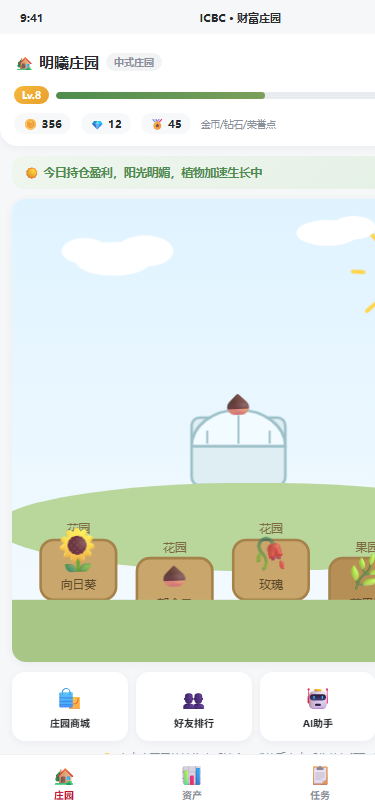
\includegraphics[width=0.31\textwidth]{img/manor.png}\hfill
  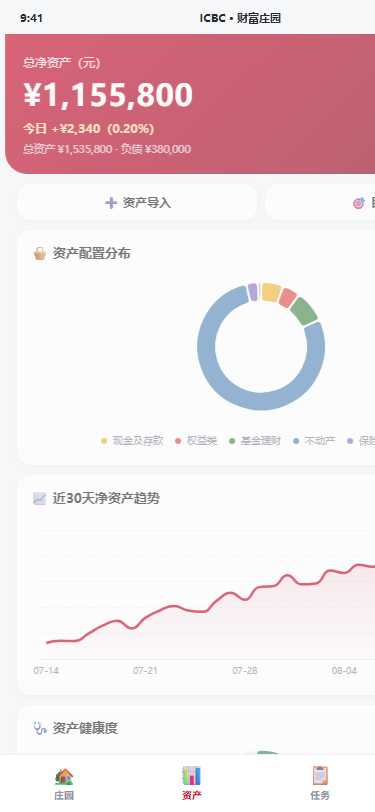
\includegraphics[width=0.31\textwidth]{img/assets.png}\hfill
  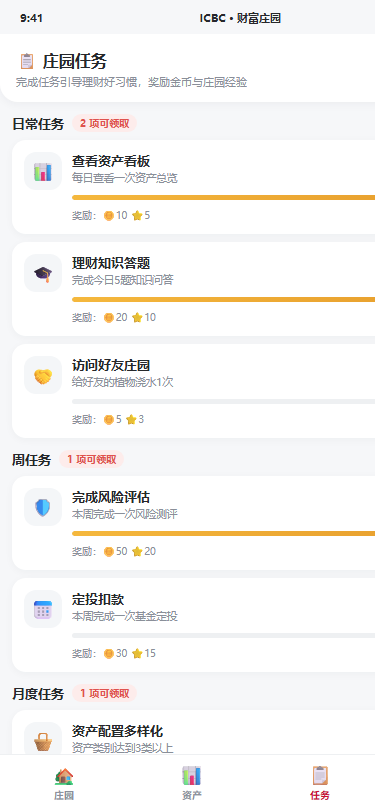
\includegraphics[width=0.31\textwidth]{img/tasks.png}
  \\[0.5em]
  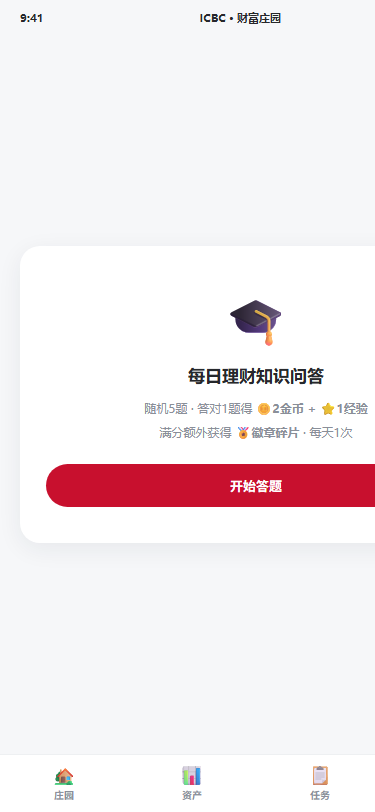
\includegraphics[width=0.31\textwidth]{img/quiz.png}\hfill
  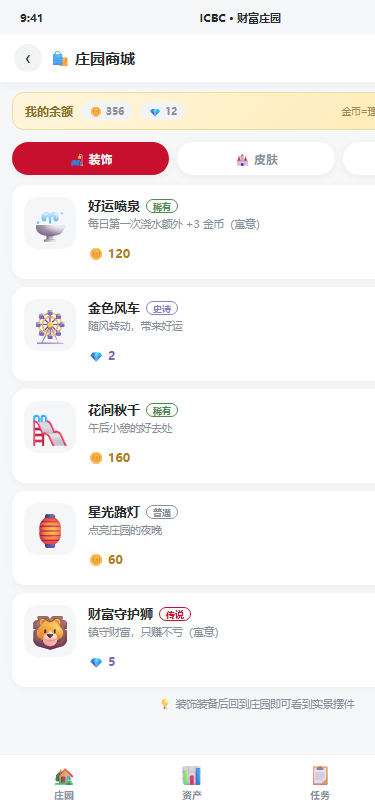
\includegraphics[width=0.31\textwidth]{img/shop.png}\hfill
  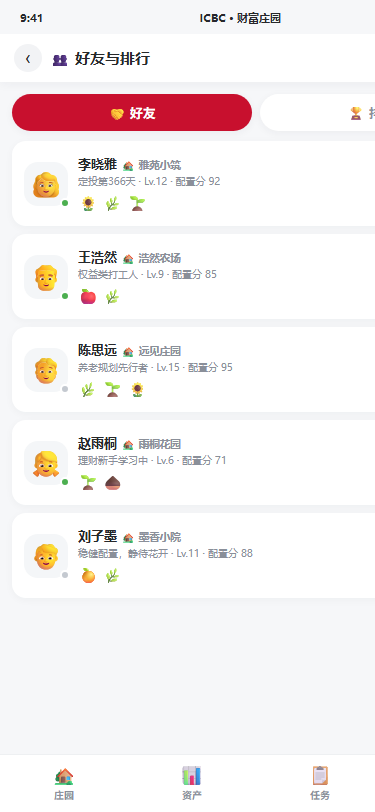
\includegraphics[width=0.31\textwidth]{img/social.png}
  \caption{财富庄园演示原型（上排左起：庄园主页、资产看板、任务中心；
          下排左起：知识答题、装扮商城、好友与排行）}
  \end{figure}
}{
  \begin{center}
  \fbox{\parbox{0.82\textwidth}{\centering\vspace{2.5em}
  \large 演示截图占位区\par\vspace{0.8em}
  \small 运行演示原型后，执行 \texttt{wealth-manor/scripts/capture-demo.mjs}
  自动生成截图并重新编译本文档即可插入。\par\vspace{2.5em}}}
  \end{center}
}

\subsubsection{演示环境与后续演进}
原型演示环境为本地浏览器（桌面浏览器以手机框呈现，亦可整屏运行）。
生产演进路径为：Mock数据层 $\rightarrow$ 对接工行真实账户/产品/行情接口
$\rightarrow$ Cocos Creator 游戏引擎替换SVG场景 $\rightarrow$ 接入行内AI平台
与大模型 $\rightarrow$ 灰度发布。

\end{document}
